\section{Abstract Syntax Tree}

\begin{itemize}
  \item The Abstract Syntax Tree (AST) is a tree-like data structure representing the essential syntactic structure of a program’s source code.
  \item It is constructed by the syntax analysis phase of a compiler, immediately after lexical analysis.
  \item The AST serves as a crucial intermediate representation for subsequent compiler phases: semantic analysis, intermediate code generation, and code optimisation.
  \item It abstracts away inessential concrete syntax details (e.g.\ parentheses, semicolons) to focus on core syntactic and semantic information \cite{aho2007compilers}.
\end{itemize}

\begin{figure}[hb!]
    \centering
    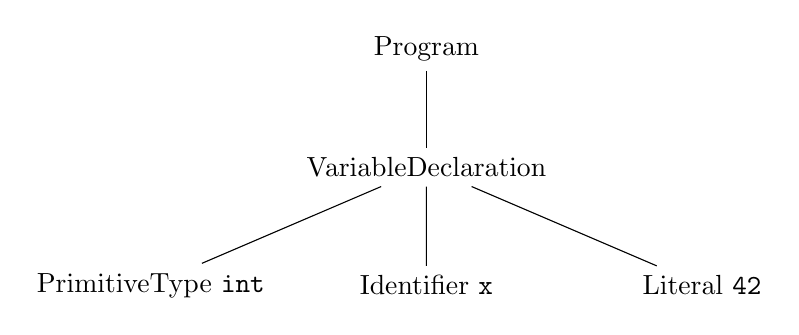
\begin{tikzpicture}[level distance=1.5cm, sibling distance=3.5cm]
      \node {Program}
        child { node {VariableDeclaration}
          child { node {PrimitiveType \texttt{int}} }
          child { node {Identifier \texttt{x}} }
          child { node {Literal \texttt{42}} } };
    \end{tikzpicture}
    \caption{AST of the program \texttt{int x = 42;}}
    \label{fig:ast-tinyc}
\end{figure}

\subsection{Key Components}

In an AST, each node represents a construct occurring in the source code \cite{aho2007compilers}. These constructs can include operators (e.g.\ addition, subtraction), variables, control flow statements (e.g.\ if-then-else, loops), function calls, and literals. The children of a node represent its components or operands. For instance, in an AST for the expression \texttt{2 + (z - 1)}, the root node represents the addition operation (\texttt{+}), with two children: one for the literal \texttt{2}, and one for the subtraction operation (\texttt{-}), which in turn has children \texttt{z} and \texttt{1}. Each node stores information about its construct type and related data (e.g.\ variable names, literal values), encoding hierarchical relationships and operator precedence \cite{aho2007compilers}.

\subsection{Abstraction from Concrete Syntax}

The AST abstracts away inessential concrete syntax details present in a parse tree \cite{aho2007compilers}. It omits grouping parentheses, statement-terminating semicolons, and parsing-only non-terminals, retaining only the constructs needed for semantic understanding. By eliminating syntactic sugar and focusing on semantic content, the AST provides a cleaner, more manageable structure for semantic analysis and code generation \cite{aho2007compilers}.

\subsection{Further Compiler Stages}

As an intermediate representation, the AST bridges initial code analysis and later compiler phases. It underpins semantic analysis—checking types, scopes, and other constraints—by providing a traversable structure. The AST also forms the basis for generating machine-independent intermediate code and enables code optimisation techniques through its well-defined hierarchy. A carefully designed AST thus directly impacts the efficiency and correctness of generated target code \cite{aho2007compilers}.

\section{Conclusion}

This chapter has explored the fundamental theoretical concepts that underpin the frontend of a compiler. We have examined the principles of formal languages, which provide the mathematical framework for defining the syntax of programming languages. We have also discussed the compilation process as a sequence of phases, with a particular focus on lexical analysis, the process of breaking down the source code into tokens, and syntax analysis, which involves parsing these tokens according to the language's grammar. Finally, we delved into the design and importance of Abstract Syntax Trees, which serve as a crucial intermediate representation of the program's structure for subsequent compiler stages. These theoretical concepts are interconnected and collectively form the essential foundation for the design and implementation of efficient and reliable compiler frontends. The principles discussed here will be directly applicable and further elaborated upon in the subsequent chapters, where we will explore their application in the specific context of the \texttt{tinyC} compiler frontend.